\documentclass[a4paper]{article}
\usepackage{isabelle,isabellesym}

% further packages required for unusual symbols (see also
% isabellesym.sty), use only when needed

%\usepackage{amssymb}
  %for \<leadsto>, \<box>, \<diamond>, \<sqsupset>, \<mho>, \<Join>,
  %\<lhd>, \<lesssim>, \<greatersim>, \<lessapprox>, \<greaterapprox>,
  %\<triangleq>, \<yen>, \<lozenge>

%\usepackage{eurosym}
  %for \<euro>

%\usepackage[only,bigsqcap]{stmaryrd}
  %for \<Sqinter>

%\usepackage{eufrak}
  %for \<AA> ... \<ZZ>, \<aa> ... \<zz> (also included in amssymb)

%\usepackage{textcomp}
  %for \<onequarter>, \<onehalf>, \<threequarters>, \<degree>, \<cent>,
  %\<currency>

\usepackage[utf8]{inputenc}
\usepackage{makeidx}
\usepackage{graphicx}
\usepackage{tabularx}
\usepackage{amssymb}
\usepackage{amsmath}
\usepackage{color}
\usepackage{booktabs}
\newcommand{\todo}[1]{\textcolor{red}{TODO: #1}}
\usepackage{pifont}
\usepackage{moeptikz}
\DeclareUnicodeCharacter{2713}{\ding{52}}
\DeclareUnicodeCharacter{2717}{\ding{56}}
\DeclareUnicodeCharacter{00D7}{\ensuremath{\times}}%               ×
\usepackage{flushend}
\usepackage{stmaryrd}
\usepackage{mathtools}
\hyphenation{swit-ches}
\usepackage{alphabeta}
\usepackage{url}
\usepackage{tikz}
\usetikzlibrary{calc,positioning}
\widowpenalty100000
\clubpenalty100000
\usepackage{pbox}
\usepackage{subcaption}
\usepackage{listings}
\lstset{breaklines=true,numbers=left,numberstyle=\tiny\color{gray},basicstyle=\footnotesize\ttfamily}
\usepackage{pgfplots}
\twocolumn
\columnsep 2pc          %    Space between columns
\textwidth 42pc         % Width of text line.
\oddsidemargin 4.5pc
\evensidemargin 4.5pc
\advance\oddsidemargin by -1in  % Correct for LaTeX gratuitousness
\advance\evensidemargin by -1in % Correct for LaTeX gratuitousness
\marginparwidth 0pt             % Margin pars are not allowed.
\marginparsep 11pt              % Horizontal space between outer margin and
\emergencystretch=3cm


% this should be the last package used
\usepackage{pdfsetup}

% urls in roman style, theory text in math-similar italics
\urlstyle{rm}
\isabellestyle{it}

% for uniform font size
%\renewcommand{\isastyle}{\isastyleminor}

\usepackage[english]{babel}
% for \frqq (whatever that actually is)

\begin{document}

\title{Verified Migration of Linux Firewalls to SDN}
\author{Julius Michaelis and Cornelius Diekmann}
\maketitle

\begin{abstract}
	We present a system that transforms the main routing table and \texttt{FORWARD} chain of iptables of a Linux-based firewall into a set of static OpenFlow rules.
	Our implementation is verified against a model of a simplified Linux-based router and we can directly show how much of the original functionality is preserved.
\end{abstract}

%\tableofcontents

% sane default for proof documents
\parindent 0pt\parskip 0.5ex

\section{Introduction}
The service requirements for computer networks have grown more and more complicated since networks first emerged, causing serious problems for their operators.
To mitigate the rising complexity and help innovation in networks the \emph{Software Defined Networking} (SDN) approach has been invented.
It gives network administrators a more centralized and easy to overview way of configuring their network. 

This paper focuses on one problem of the SDN approach: There is a lot of existing configuration in ``legacy'' configuration languages.
Early SDN approaches such as SANE~\cite{casado2006sane} or 4D~\cite{greenberg2005clean} did not account for this and required network operators to start their configuration from a clean slate.
Given the overall tendency that existing software and configuration is usually left untouched as far as possible, this is obviously unacceptable in many cases.
The currently most promising variant of SDN, \emph{OpenFlow}~\cite{mckeown2008openflow}, accounts for this by allowing devices to primarily process traffic in an SDN mode, and giving the configuration in that mode a way to hand packets off to the traditional, device-dependent processing chain.
While OpenFlow thereby fulfils the requirements of backwards compatibility, it also means that its users will have one more configuration format around that needs to be maintained.
The hybrid OpenFlow approach thus not necessarily reduces the complexity of maintaining a network or verifying its correctness.

This paper uses a different approach to handle legacy configuration: convert the legacy configuration to a format that can be handled with OpenFlow.
Since it is impossible to understand and convert an arbitrary configuration format, we focused on the configuration of a \emph{Linux}-based firewall, including routing and firewall/\emph{iptables} configuration.
Furthermore, we have decided to convert the configuration to a set of static OpenFlow rules that can be inserted on deployment and do not require a controller.

The rest of this paper is organized as follows.
Since we require models of both an OpenFlow switch and a Linux firewall, we include an extensive survey of models of networking boxes and how they are used in Section~\ref{sec:surv}.
The models we created, and how the translation of configuration of one to the other works is explained in Section~\ref{sec:conv}.
An evaluation of our system based on \emph{mininet}~\cite{lantz2010network} simulations and real configuration samples is shown in Section~\ref{sec:eval}.

\section{Model Survey}\label{sec:surv}
We continue with the survey of different networking device models.
Section~\ref{sec:sw} surveys link layer switches, Section~\ref{sec:rtr} routers, Section~\ref{sec:sdn} SDN switches, and Section~\ref{sec:fw} Firewalls.
Section~\ref{sec:pl} looks at models of devices that do not only provide a single function.
Additionally, Section~\ref{sec:bsw} shows the \emph{big switch model}.
This survey has already appeared in~\cite{michaelis2016middlebox} together with some additional parts.
\begin{figure*}
	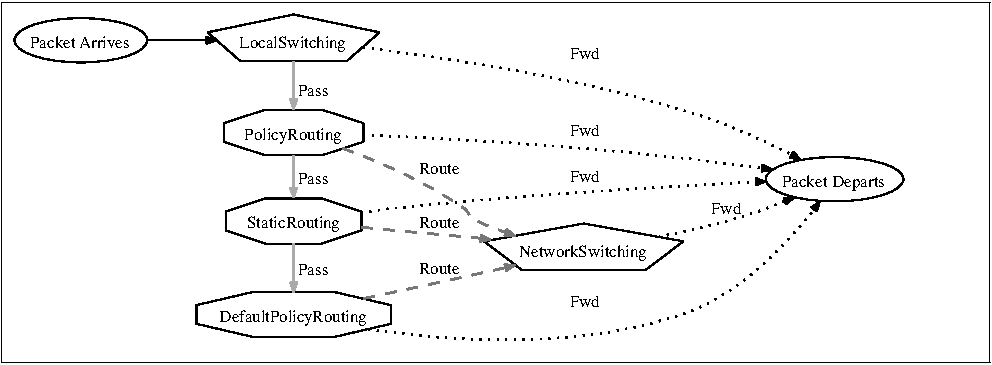
\includegraphics{fig/rtr.pdf}
	\caption{Margrave's router model, taken from \cite{nelson2010margrave}.}
	\label{fig:margraverouter}
\end{figure*}
\subsection{Link Layer Switches}\label{sec:sw}
When considering only the basic switching functionality, Link layer switches become relatively simple devices.
They neither offer many opportunities for modeling, nor are they very interesting as a target for verification, since most switches simply have no configuration to verify.
Accordingly, there is not much material in the related literature.

There is one problem that arises when verifying networks that contain switches among other devices.
Switches are stateful devices, while some verification systems do not support state.
A simple modeling solution for that is presented in Header Space Analysis~\cite{kazemian12header}:
\begin{quote}
	When we generated box transfer functions, we
	chose not to include learned MAC address of end hosts.
	This allowed us to unearth problems that can be masked
	by learned MAC addresses but may surface when learned
	entries expire.
\end{quote}
While this modelling decision has consequences for the models of a variety of devices, it implies that switches are always in their learning phase, i.e.\ are effectively replaced by broadcast devices.

\subsection{Routers}\label{sec:rtr}

For this section, we will focus solely on layer 3 forwarding.
%Since the process is relatively simple we have kept this section short.

While Margrave \cite{nelson2010margrave} is originally a tool for the analysis of firewalls, it also has a detailed understanding of the packet forwarding process in Cisco IOS to be able to accurately perform its tasks.
The model that Margrave uses is shown in Figure \ref{fig:margraverouter}.
The process of forwarding is described as follows.
First, packets destined to locally attached subnets are filtered out and directly forwarded.
All other packets are subjected to routing.
The second step is thus to handle policy routing --- packets with special routing rules that do not only depend on the destination address but e.g., on the source address, too.
The third step is to consider statically configured routes.
All remaining packets are processed using the default policy.

A more abstract model of routing is presented by Xie \emph{et al.}~\cite{xie2005static}.%
\footnote{The Anteater tool~\cite{mai2011debugging} is based on this work.}
They model a network of routers to be an annotated graph $(V,E,\mathcal{F})$ where the nodes $V$ represent the routers, $E$ contains two directed edges for each physical link, and the edge labels $F_{u,v} \in \mathcal{F}$ express which packets are allowed to flow over an edge $u,v$.
%\footnote{Note that this model can not represent two physical links between two routers.}
The routing process is modelled using $\mathcal{F}$:
a flow over an edge $u,v$ will only be permitted by $F_{u,v}$ if the router $u$ has a route to $v$ for that specific flow.

To summarize, the Margrave's model \cite{nelson2010margrave} describes the routing process while the model in \cite{xie2005static} abstracts it away to be a property of a graph.

\subsection{SDN Switches}\label{sec:sdn}
This section surveys selected works on switches in software defined networking (SDN).
Various approaches to SDN exist.
This section focuses on OpenFlow~\cite{mckeown2008openflow} since it is currently the most actively researched variant.
We assume that the reader is familiar with its basics.
While it could be said that the OpenFlow switch specification~\cite{specification15} itself is based on a model of a generic networking device, we are not going to explore this and instead examine models of OpenFlow switches.
We will continue to denote OpenFlow switches as switches in this section for succinctness.
The term \emph{datapath element} would be more accurate since the switches can take arbitrary functions.

Guha \emph{et al.}~\cite{guha2013machine} present a fully machine-verified implementation of a compiler for the NetCore controller programming language.
For this purpose, they give a detailed model of an OpenFlow switch that adheres closely to version 1.0 of the OpenFlow switch specification \cite{specification10}, including packet processing and switch-controller interaction.
We will examine the most important details and begin with the flow table evaluation semantics:
Guha \emph{et al.} dedicate significant attention to how a packet is matched against a flow table entry.
Their main concern there is related to behavior that was only made explicit in later versions of the specification, e.g.\ \cite[§7.2.3.6]{specification15}:
\begin{quote}
	The presence of an [OpenFlow match] with a given [type] may be restricted based on the presence or values
	of other [matches], its prerequisites.
	Matching header fields of a protocol can only be done if the OpenFlow match explicitly matches the corresponding protocol.
\end{quote}
For example, to match an outgoing SSH connection, a match must check for at least layer 4 destination port 22, layer 4 protocol TCP, and layer 3 protocol IP.
If only the match for layer 4 destination port is included, some implementations of an OpenFlow switch return an error as required by the specification~\cite[§7.2.6.7]{specification15}.
Others, including the reference implementation~\cite{openvswitch}, silently drop them, which has led to several severe bugs, according to \cite{guha2013machine}.
Guha \emph{et al.} specify their packet matching semantics to only evaluate matches when a previously executed match on the preconditions has assured that the necessary header fields are present.

Next, they specify a flow table to be a multiset of triples of priority, a match condition, and a multiset of output ports.
Although a multiset allows for uncountably many flow table entries instead of a bounded number thereof, the implications for the validity of the model are minimal.
The semantics $\llbracket \mathit{FT} \rrbracket~\mathit{pt}~\mathit{pk} \rightsquigarrow (o,c)$  for evaluating such a table is shown in Figure \ref{fig:guhafts}.
\begin{figure}
	\centering
	\fbox{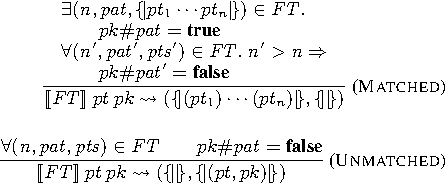
\includegraphics{fig/ofts.pdf}}
	\caption{Flow table semantics by Guha \emph{et al.}, taken from \cite{guha2013machine}.}
	\label{fig:guhafts}
\end{figure}
The semantics describes the decision for a flow table $\mathit{FT}$ and a packet $pt$ arriving on a port $p$.
It can specifiy to forward the packets on the port set $o$ or to send the messages $c$ to the controller.
The operator $\#$ matches a packet against a rule.
Note that this semantics is nondeterministic:
	if there are multiple matching flow table entries with the same priority, it can be said that all of their actions are executed nondeterministically.
This is used to model the fact that the specification~\cite[§3.4]{specification10} says that the switch is free to choose any order between overlapping flow entries.
For this paper, we have verified that determinism can be enforced by adding the following precondition on the flow table:
\begin{align}
	&\forall\!\left(n,\mathit{pat},\mathit{pts}\right) \in \mathit{FT}.~\forall\!\left(n',\mathit{pat}',\mathit{pts}'\right) \in \mathit{FT} \setminus \left\{\left(n,\mathit{pat},\mathit{pts}\right) \right\}.& \nonumber\\
	&n = n' \Longrightarrow \nexists \emph{pk}.~\emph{pk}\#\emph{pat} \wedge \emph{pk}\#\emph{pat}'\text{,}&
\end{align}
i.e.\ for two rules with the same priority, no packet matches both. Note that this is slightly stronger than necessary to make the semantics deterministic: overlapping entries could be shadowed by a rule with higher priority.

Guha \emph{et al.} also specify a semantics for the message processing and passing between switches and controllers.
They model it as an inductively defined relation on the states of switches, controller(s) and links between them.
The semantics of this is comparatively large: its 12 rules span an entire page.
There is one important modelling detail that can be singled out:
Switches are modelled as a tuple of their unique identifier, their ports, one flow table, and four message queues, one for each combination of in/out and controller/switch to switch.
These message queues are multisets.
On the receipt of a message through a link, or when obtaining a message through processing at a switch, the message is first enqueued in one of these queues.
The semantics is non-deterministic and allows to accumulate arbitrary many messages and dequeue them in an arbitrary order.
This models the option for switches to reorder messages.
The only exception is a \emph{BarrierRequest}, which is never enqueued but, given that the input queue is empty, directly processed.
It can thus be used to ensure that all messages have been sent before it is processed.

Orthogonal to the work of Guha \emph{et al.} stands VeriCon~\cite{ball2014vericon}.
It is not a verified compiler for controller programs but a verifying tool for controller programs.
It does not have a detailed model of single switches against which it verifies the output of its compiler.
Instead, it checks its result on a high-level model of a network of switches.
Its authors, Ball \emph{et al.}, begin by presenting a simple example programming language for controllers, called CSDN, and give a formal semantics for this language.
VeriCon allows to prove correctness of programs within these semantics but it does not establish the correctness of the compiler.
VeriCon takes three inputs: a CSDN program, a topology invariant, and a correctness condition.
The topology invariant allows to limit the possible changes in topology, e.g., the user can define that they will always ensure that no path in the network has more than 3 hops.
The correctness condition is then verified to hold for all possible states and topology changes.
To achieve that, VeriCon uses the following high-level model of a network of switches: Its state is modelled as 5 relations.
The first relation contains the links between switches, or switches and hosts,
the second one all paths that are possible over those links.
These two relations are mainly used to formulate topology invariants.
The third relation $S.\mathit{ft}\left(\mathit{Src}\rightarrow\mathit{Dst}, I\rightarrow O\right)$ records whether switch $S$ has a rule in its forwarding table to forward packets from host $\mathit{Src}$ to $\mathit{Dst}$ from input port $I$ to output port $O$.
Similar to that $S.\mathit{send}\left(\mathit{Src}\rightarrow\mathit{Dst}, I\rightarrow O\right)$ records whether such a packet has actually been sent.
Lastly, the relation $S.\mathit{rcv}^\mathit{this}\left(\mathit{Src}\rightarrow\mathit{Dst}, I\right)$ models whether a packet has been received at input port $I$.
With these, given a desired postcondition $Q$, VeriCon can compute the weakest precondition $\mathit{wp}\llbracket c\rrbracket(Q)$ for executing a command $c$ in CSDN.
For example:
\begin{align}
	&\mathit{wp}\left\llbracket \mathit{pktIn}\left(s,p,i\right) \Rightarrow c\right\rrbracket\left(Q\right) \coloneqq \nonumber\\
	&\left(s.\mathit{rcv}^\mathit{this}\left(p,i\right) \wedge s.\mathit{ft}\left(p,i\rightarrow o\right)\right) \Longrightarrow \mathit{wp}\llbracket c\rrbracket\left(Q\right)\text{.}&
\end{align}
This is the precondition semantics for the event handler specification $\mathit{pktIn}(s,p,i) \Rightarrow c$. 
In the event of receiving a packet $p$ at port $i$ of switch $s$, $c$ is executed.
The semantics expresses the following: given that such a packet is actually received and a forwarding rule is installed, the handle has to satisfy the weakest precondition of its command.

Similar to VeriCon is NICE \cite{canini2012nice}.
It uses model checking and other techniques to verify the correctness of a controller program at runtime.
It models an SDN as a system of stateful ``components'' that communicate in a first-in first-out manner.
Communication between the components is, among other things, modelled by state transitions in the system.
The controller programs are modelled accordingly: as a set of event handlers that trigger state changes in the controller.
For model checking, NICE executes these handlers to explore the state space and see if any of the transitions can violate correctness invariants.

NICE notes that, for model checking, it would also need to explore the state space of the switches.
Since even the reference implementation Open vSwitch \cite{openvswitch} has multiple hundred KB of state when executed, this is not directly feasible.
NICE thus presents a simple model of a switch with a reduced amount of state.
A switch is modelled as a set of communicating channels, two state transitions and a single flow table.
Except for the control channel, which operates strictly in a first-in first-out manner, these channels may also drop or reorder messages\footnote{Note the difference to \cite{guha2013machine} where the control channel does also not operate in a first-in first-out manner and can reorder messages.}.
On the receipt of at least one message, a state transition is executed.
To reduce the amount of state transitions necessary, all packets present in a state are modelled as being processed as a single transition.
NICE also makes an important remark on the flow table: two flow tables can be syntactically different, i.e.\ have a different entry structure, but be semantically equivalent, i.e.\ lead to the same forwarding decisions.
This observation is true for all three models here.
For example, a table that contains only exact flow matches (flow entries without any wildcards) makes decisions independent of the priority of the rules (i.e.\ the order in which they are considered)\footnote{Assuming that the switch does not accept overlapping rules.}.
NICE uses heuristics to merge semantically equivalent states.

\subsection{Firewalls}\label{sec:fw}
The term firewall is used for a diverse variety of devices and software.
Devices by different vendors, such as Cisco, Sun Microsystems, or Sophos have a largely different set of features and purposes.
Even the Linux kernel has two different firewall implementations (iptables and nftables).
This means that a large number of different models exists.
Nevertheless, a common principle can be factored out: most firewalls and all models considered here consist of rules, which in turn consist of at least a match and an action.
The match decides whether the action is to be applied to a given packet.
The firewalls' types differ in how rules are organized, i.e.\ in which order they are applied, and what kind of match expressions and actions are supported.
Another detail of interest is how connection state tracking is modelled, i.e.\ how packets that belong to established connections are treated differently from packets for new connections.
Many real world firewalls begin by accepting packets that belong to or are related to an established connection.
Finding a simple but powerful model for state is hence important.

Accompanying a model of a firewall, there always has to be a model of packets on which the firewall operates, albeit this is often left implicit.
One of the few works that explicitly specifies the packet model is \cite{brucker2007test}:
\begin{align}
	&\left(α, β\right) \mathit{packet} \coloneqq \nonumber\\
	&\left(id × protocol × α\, src × α\, dest × β\, content\right) \text{.}
\end{align}
This can be read as: given arbitrary types $α$ and $β$, a packet consists of a record of a unique identifier, the used protocol (http, ftp, …), a source and destination address of type $α$ and packet content of type $β$.%
\footnote{Brucker et Wolff later specify $α$ to be a four-tuple of integers to represent the IP-address in dotted-decimal notation and a port, also represented by an integer (i.e.\ a number from $\mathbb{Z}$).}
It is obvious that this format does not model real packets very closely, since neither the used (application layer) protocol is usually stated directly, nor is every connection associated with a unique ID.
Nevertheless, the ID hints to how state is modelled by Brucker et Wolff in~\cite{brucker2007test}.
They model state by allowing the match to consider a list of all packets that the firewall has accepted so far.
The ID can be used to determine if a packet is the first of its connection.

A less complicated model of state, which is also based on the packet format, can be found in ITVal~\cite{marmorstein2005tool} (however, not in a strongly formal manner).
Whether a packet is part of an established connection is simply treated to be another packet field.
The theory files accompanying \cite{diekmann2015semantics} contain a proof that that model is not weaker than querying an internal state table when performing a stateful match.

The packet model is often tightly tied to which types of match expressions the firewall supports.
A very common subset that can be found in many real firewalls and models is to support equality matches on (OSI) layer 4 protocol, source, destination (``ports''), the physical ingress port and additionally prefix matches on the layer 3 addresses.
Some models extend this by fields for TCP flags~\cite{marmorstein2005tool,yuan2006fireman}%
, or connection state~\cite{brucker2007test,nelson2010margrave}.

Besides the set of supported match expressions, firewalls and models also differ in how these expressions can be combined and how these combinations are represented.
Margrave~\cite{nelson2010margrave} supports conjunctions of disjunctions, i.e.\ it allows to specify several possible values for one field and allows combining fields while requiring all of them to match.
\emph{Iptables Semantics}~\cite{diekmann2015semantics} by Diekmann \emph{et al.} allows for more complicated expressions:
given \emph{match} is a match on a single field, it supports the following match expressions \emph{mexpr}:
\begin{align}
	\mathit{mexpr} \coloneqq \mathit{match}~|~\neg\mathit{mexpr}~|~\mathit{mexpr}\wedge\mathit{mexpr}~|~\text{\texttt{True}}
\end{align}
This model is a superset of what iptables supports:
	iptables supports negation of matches only on the lowest level, i.e.\ it only supports constructing $\neg\mathit{match}$ but not $\neg\mathit{mexpr}$.
This is an example (but not the only one) of a model that could have been easily made to mirror a system more closely but instead was made more powerful.
In this case, $\mathit{mexpr}$ allows to express arbitrary boolean functions, which can be used to compute the expression for packets that are not matched by a rule.

Packet and match models that are tailored to be suitable for the implementation of an analysis can be found in FIREMAN~\cite{yuan2006fireman} and ITVal~\cite{marmorstein2005tool}.
FIREMAN models a packet as a vector of bits that represent its header.
Match expressions are boolean expressions that can be efficiently represented by \emph{Reduced Ordered Binary Decision Diagrams (ROBDD)}~\cite{bryant1986graph}.
ITVal~\cite{marmorstein2005tool} extends this to \emph{MDDs}~\cite{liaw1992obdd}, a structure that is similar to a \emph{ROBDD} but allows continuous values for its variables.
Consequently, ITVal models packets as the vector of bytes that represent source and destination for IP address and layer 4 port.
Additionally, it keeps separate fields for the layer 4 protocol type, the TCP flags and the connection states.
Each byte and field is then represented by one level in the MDD.
Figure~\ref{fig:itvalmdd} shows an example of how an MDD is used to match a single IP prefix.
The purpose of this subdivision of the packet header is to create a balance between too many levels and too much information on a single level of the MDD.
\begin{figure}
	\centering
	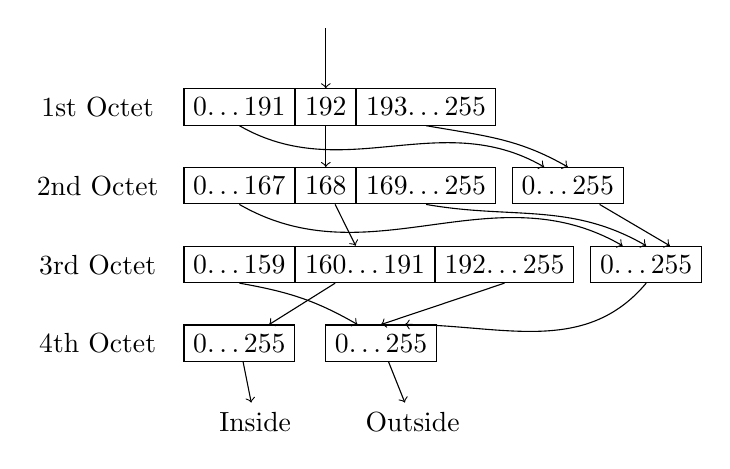
\begin{tikzpicture}[
			bloc/.style={
				node distance=0,
				draw,
				rectangle,
				anchor=west,
				text height={height("192…255")},
			},
			fbloc/.style={
				bloc,
				node distance=1.8cm,
			}
		]
		\node(c1){1st Octet};
		\node[fbloc,right of=c1] (c11) {0…191} node[bloc] (c12) at (c11.east) {192} node[bloc] (c13) at (c12.east) {193…255};

		\node[below of=c1](c2){2nd Octet};
		\node[fbloc,right of=c2] (c2a1) {0…167} node[bloc] (c2a2) at (c2a1.east) {168} node[bloc] (c2a3) at (c2a2.east) {169…255};
		\node[fbloc,right of=c2a3] (c2b1) {0…255};

		\node[below of=c2](c3){3rd Octet};
		\node[fbloc,right of=c3] (c3a1) {0…159} node[bloc] (c3a2) at (c3a1.east) {160…191} node[bloc] (c3a3) at (c3a2.east) {192…255};
		\node[fbloc,right of=c3a3] (c3b1) {0…255};

		\node[below of=c3](c4){4th Octet};
		\node[fbloc,right of=c4] (c4a1) {0…255};
		\node[fbloc,right of=c4a1] (c4b1) {0…255};

		\coordinate[below of=c4](c5);
		\node[right of=c5, node distance=2cm](in) {Inside};
		\node[right of=in, node distance=2cm](out) {Outside};

		\coordinate[above of=c12] (c02);
		\draw (c02) edge[->] (c12);

		\draw (c11.south) edge[->,out=-30,in=150] ([xshift=-.3cm]c2b1.north);
		\draw (c13.south) edge[->,out=-10,in=150] (c2b1.north);
		\draw (c12.south) edge[->] (c2a2.north);
		
		\draw (c2a1.south) edge[->,out=-30,in=150] ([xshift=-.3cm]c3b1.north);
		\draw (c2a3.south) edge[->,out=-10,in=150] (c3b1.north);
		\draw (c2b1) edge[->] ([xshift=.3cm]c3b1.north);
		\draw (c2a2) edge[->] (c3a2);
		
		\draw (c3a1.south) edge[->,out=-10,in=150] ([xshift=-.3cm]c4b1.north);
		\draw (c3a3.south) edge[->] (c4b1.north);
		\draw (c3b1.south) edge[->,out=-130,in=0] ([xshift=.3cm]c4b1.north);
		\draw (c3a2) edge[->] (c4a1);

		\draw (c4b1) edge[->] (out);
		\draw (c4a1) edge[->] (in);

	\end{tikzpicture}
	\caption{Example of how ITVal~\cite{marmorstein2005tool} would represent a match for 192.168.160.0/19, given that the packet consists only of a single IP address to match on.}
	\label{fig:itvalmdd}
\end{figure}

After considering the match of a rule, the action has to be modelled.
The common subset of actions that can be found in all models we analyzed is to either let packets pass the firewall or to stop them.
Iptables supports a number of other actions that are directly executed, such as \texttt{LOG}, which will generate debug output but have no effect on forwarding, or \texttt{REJECT}, which will stop the packet and additionally send an error message.
The semantics by Diekmann \emph{et al.}~\cite{diekmann2015semantics} shows a way to translate action types with behavior unkown to the system back to only forwarding or discarding the packet.
The model of actions given by Brucker \emph{et} Wolff~\cite{brucker2007test}, allows for something more complicated:  the action returns a packet.
This allows to model packet modification by firewall rules.

The last important property of a firewall model is how rules are combined to form the firewall.
Most models can be categorized to either use what Yuan \emph{et al.}~\cite{yuan2006fireman} call the \emph{simple list model}~(used e.g.\ in \cite{nelson2010margrave}) and the \emph{complex chain model}~(used e.g.\ in \cite{marmorstein2005tool}).
The list model states that the firewall rules are written as one list that is traversed linearly.
Each rule either applies and the execution terminates or the execution continues with the next rule.
The chain model extends this by allowing for multiple lists and the possibility to conditionally jump to the start of such a list and to conditionally return to the origin of the jump.
Diekmann \emph{et al.}~\cite{diekmann2015semantics} formalized both and present a translation from the chain model to the list model. 

If a firewall is an actual networking device, it also needs to decide on which port to forward packets, i.e.\ become a switch or router additionally to its firewall function.
This type of combined functionality is considered in the next section.
\subsection{Complex devices}\label{sec:pl}
Real network devices often fulfil more than one of the functions described above.
A common example of this is a Cisco IOS router, which is usually configured with both an ACL (i.e.\ its firewall function) and routing information.

An important insight is that these functions usually have very little or no relevant shared state.
The key implication of this is that the different stages of such a system can be analyzed separately and then \emph{pipelined} together.
In the example of the IOS router, this would mean to first analyze the incoming ACL, then the routing configuration and then the outgoing ACL.

Dobrescu and Argyraki~\cite{dobrescu2014software} have realized that this holds true even for controller software that is written for SDN switches.
When attempting verification of software in general, one has to deal with the path explosion problem.
By dividing a network system into $m$ independent elements with maximally $n$ branches each, pipelined analysis can reduce the amount of paths that has to be analyzed exponentially from $\mathcal{O}\left(2^{mn}\right)$ to $\mathcal{O}\left(m2^n\right)$.
Combined with further optimization for relevant data structures and symbolic computation, their tool \emph{ClickVerifier} is able to verify controller programs.
Dobrescu and Argyraki make an explicit point of using the pipeline model only to explain why their system has the desired performance.
For the verification, the actual generated controller program bytecode is passed to the analysis engine S$^2$E~\cite{chipounov2009selective} to avoid any abstraction errors that might happen when modeling OpenFlow switches.

Another interesting instance of the pipelining model can be found in the tool Margrave by Nelson \emph{et al.}~\cite{nelson2010margrave}.
\begin{figure*}
	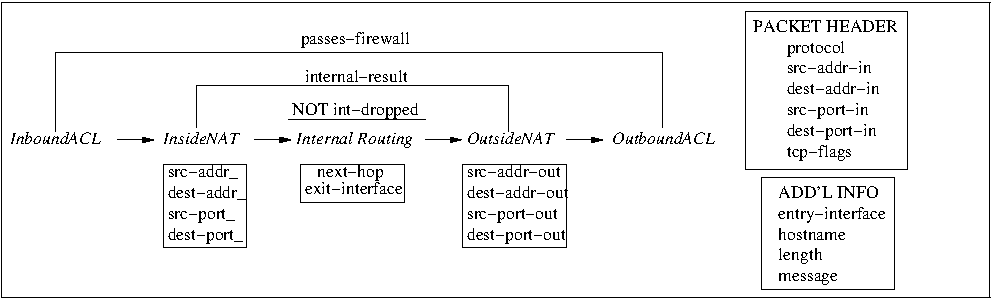
\includegraphics{fig/pipeline.pdf}
	\caption{Margrave's decomposition of IOS configurations, taken from \cite{nelson2010margrave}}
	\label{fig:margravedecomp}
\end{figure*}
A schematic representation of how it is used to decompose a Cisco IOS configuration can be found in Figure \ref{fig:margravedecomp}.
Each element of the pipeline is used to provide the further elements of the pipeline with necessary information to continue the analysis, e.g., the \emph{Internal Routing} step is used to decide which outbound NAT and ACLs apply.

A very similar approach to this is taken in Hassel, the tool that implements Header Space Analysis by Kazemian \emph{et al.}~\cite{kazemian12header}.
Hassel translates dumped Cisco IOS configurations into functions represented in a model on which symbolic computation is possible.
Representing the full function of a router with a single function of this model would result in very large representations.
The transfer through one Cisco IOS router is thus modelled as traversing three layers in the model, one input ACL and VLAN untagging step, one routing step, and one output processing step.
The difference to how Margrave uses the pipeline model is that Header Space Analysis reuses the exact same model for each step.

This solution of size reduction is also applied by Exodus~\cite{nelson2015exodus}.
It translates Cisco IOS configurations into controller configuration for an OpenFlow switch (\emph{cf.}\ Section~\ref{sec:sdn}).
Much of the available OpenFlow capable hardware only supports a single table of matches and output ports.
Similar to the functions of Hassel, compressing the entire functionality of a Cisco switch into a single table would create very large representations through the use of cross products.
Exodus thus uses multiple switches (i.e. physically multple devices).
Their pipeline steps are, in order, VLAN untagging, input ACLs, routing, NAT, routing (2), layer 2 rewriting, output ACLs, and VLAN tagging.

\subsection{Big Switch Model}\label{sec:bsw}
While the \emph{big switch model} is not strictly speaking a model of a networking device but a model of the entire network, we feel that it is important enough to mention it here.
It is used in various places, first and foremost in SDN \cite{casado2010virtualizing,kang2013optimizing,monsanto2013composing} programming languages, but also e.g., for network verification~\cite{anderson2014netkat}.
The general idea is that a network or subnetwork of switches, routers, firewalls displays a forwarding behavior to all attached devices that are not part of the subnetwork.
The subnetwork usually has a complicated distributed configuration that defines its forwarding behavior.
Even in SDN programming languages, this state is often exposed to the programmer.
Proponents of the big switch model usually attempt to represent this state as if it was the configuration of a single switch with each of its ports representing one connection from the subnetwork to something outside of it.
The rationale for this is that a representation for the configuration of the big switch could be smaller and thus easier to understand or verify.

Anderson \emph{et al.}~\cite{anderson2014netkat} propose a slightly different interpretation of the big switch model: for a network to be an instance of the big switch model, they require that the network displays the behavior of a big learning switch, i.e.\ implements all-pairs reachability.
Since NetKAT~\cite{anderson2014netkat} allows testing the equality of two network descriptions, they formulate a formal condition for this to be true.
Showing this condition here would require explaining the formalism used by NetKAT and is thus out of scope.


% generated text of all theories
\input{session}

\section{Evaluation}\label{sec:eval}
In Section~\ref{sec:conv}, we have made lots of definitions and created lots of models.
How far these models are in accordance with the real world has been up to the vigilance of the reader.
This section attemts to alleviate this burden by providing some examples.

\subsection{Mininet Examples}
\label{sec:mnex}
\tikzset{mnod/.style={minimum width=1cm}}
\begin{figure*}
\centering
\begin{subfigure}[b]{0.45\textwidth}
\begin{lstlisting}
:FORWARD DROP [0:0]
-A FORWARD -d 10.0.2.0/24 -i s1-lan -p tcp -m tcp --sport 32768:65535 --dport 80 -j ACCEPT
\end{lstlisting}
\caption{FORWARD chain}
\end{subfigure}
\hspace{0.05\textwidth}
\begin{subfigure}[b]{0.45\textwidth}
\begin{lstlisting}
10.0.2.0/24 dev s1-wan  proto kernel  scope link  src 10.0.2.4
10.0.1.0/24 dev s1-lan  proto kernel  scope link  src 10.0.1.1
default via 10.0.2.1 dev s1-wan
\end{lstlisting}
\caption{Routing table (sorted)}
\end{subfigure}
\begin{subfigure}{\textwidth}
\begin{lstlisting}
priority=4,hard_timeout=0,idle_timeout=0,in_port=1,dl_type=0x800,nw_proto=6,nw_dst=10.0.2.0/24,tp_src=32768/0x8000,tp_dst=80,action=output:2
priority=3,hard_timeout=0,idle_timeout=0,dl_type=0x800,nw_dst=10.0.2.0/24,action=drop
priority=2,hard_timeout=0,idle_timeout=0,dl_type=0x800,nw_dst=10.0.1.0/24,action=drop
priority=1,hard_timeout=0,idle_timeout=0,in_port=1,dl_type=0x800,nw_proto=6,nw_dst=10.0.2.0/24,tp_src=32768/0x8000,tp_dst=80,action=output:2
priority=0,hard_timeout=0,idle_timeout=0,dl_type=0x800,action=drop
\end{lstlisting}
\caption{Resulting OpenFlow rules}
\end{subfigure}
\caption{Example Network 1 -- Configuration}
\label{fig:exn1}
\end{figure*}
The first example is designed to be minimal while still showing the most important properties of our conversion.
For this purpose, we used a linux firewall F, that we want to convert.
We gave it two interfaces, and connected one client each.
Its original configuration and the ruleset resulting from the translation is shown in Figure \ref{fig:exn1}. (The list of interfaces can be extracted from the routing table; \texttt{s1-lan} received port number 1.)
While the configuration does not fulfil any special function (especially, no traffic from the interface \texttt{s1-wan} is permitted), it is small enough to let us have a detailed look.
More specifically, we can see how the only firewall rule (Line 2) got combined with the first rule of the routing table to form Line 1 of the OpenFlow rules.
This also shows why the bitmasks on the layer 4 ports are necessary. If we only allowed exact matches, we would have $2^{15}$ rules instead of just one.
Line 2 of the OpenFlow ruleset has been formed by combining the default drop policy with Line 1 of the routing table.
In a similar fashion, Line 2 of the routing rules has also been combined with the two firewall rules.
However, as $10.0.2.0/24$ from the firewall and $10.0.1.0/24$ from the routing table have no common elements, no rule results from combining Line 2 and Line 2.
In a similar fashion, the rest of the OpenFlow ruleset can be explained.

We feel that it is also worth noting again that it is necessary to change the IP configuration of the two devices attached to F.
Assuming they are currently configured with, e.g., $10.0.1.100/24$ and $10.0.2.1/24$, the subnet would have to be changed from 24 to 22 or lower to ensure that a common subnet is formed and the MAC layer can function properly.

Next, we show a somewhat more evolved example.
Its topology is depicted in Figure \ref{fig:exn2}.
As before, we called the device to be replaced F.
It is supposed to implement the simple policy that the clients H1 and H2 are allowed to communicate with the outside world via HTTP, ICMP is generally allowed, any other traffic is to be dropped (we neglected DNS for this example).
We used the iptables configuration that is shown in Figure \ref{fig:exn2fw}.
The routing table is the same as in the first example network.

\begin{figure*}
\centering
\begin{subfigure}{0.4\textwidth}
\begin{tikzpicture}[node distance=2cm,scale=0.85]
\node[router,mnod](r){F};
\node[hub,mnod,left of=r](h){};
\node[server,mnod,right of=r](s1){S1};
\node[server,mnod,right of=s1](s2){S2};
\node[client,mnod,above of=h](h1){};
\node[above of=h1,node distance=1cm]{H1};
\node[client,mnod,below of=h](h2){H2};
\draw(h1) -- (h) -- (h2);
\draw(h) -- (r) -- (s1) -- (s2);
\end{tikzpicture}
\vspace{1em}
\caption{Topology}
\label{fig:exn2}
\end{subfigure}
\hspace{0.05\textwidth}
\begin{subfigure}{0.5\textwidth}
\begin{lstlisting}
:FORWARD DROP [0:0]
-A FORWARD -p icmp -j ACCEPT
-A FORWARD -i s1-lan -p tcp -m tcp --sport 1024:65535 --dport 80 -j ACCEPT
-A FORWARD -d 10.0.1.0/24 -i s1-wan -p tcp -m tcp --sport 80 --dport 1024:65535 -j ACCEPT
\end{lstlisting}
\caption{\texttt{FORWARD} chain}
\label{fig:exn2fw}
\end{subfigure}
\caption{Example Network 2}
\end{figure*}

The topology  has been chosen for a number of reasons:
we wanted one device which is not inside a common subnet with F and thus requires no reconfiguration for the translation.
Moreover, we wanted two devices in a network that can communicate with each other while being overheard by F.
For this purpose, we added two clients H1 and H2 instead of just one.
We connected them with a broadcasting device.\footnote{For the lack of a hub in mininet, we emulated one with an OpenFlow switch.}

Executing our conversion function results in 36 rules%
	\footnote{If we had implemented some spoofing protection by adding \texttt{! -s 10.0.1.0/24} to the respective rule, the number of rules would have been increased to 312. This is because a cross product of two prefix splits would occur.},
we decided not to include them here.
Comparing to the first example network, the size of the ruleset seems relatively high. This can be explained by the port matches: $1024$-$65535$ has to be expressed by 6 different matches, \texttt{tp\_src=1024/0xfc00}, \texttt{tp\_src=2048/0xf800}, \ldots, \texttt{tp\_src=32768/0x8000} (or \texttt{tp\_dst} respectively).
When installing these rules, we also have to move all of H1, H2 and S1 into a common subnet.
We chose $10.0.0.0/16$ and updated the IP configuration of the three hosts accordingly.
As discussed, the configuration of S2 did not have to be updated, as it does not share any subnet with F.
We then tested reachability for TCP 22 and 80 and ICMP.
The connectivity between all pairs of hosts (H1,H2,S1 and S2) remained the same compared to before the conversion.
This shows that the concept can be made to work.

However, the example also reveals a flaw: When substituting the more complete model of a linux firewall with the simple one in Section \ref{sec:lfw}, we assumed that the check whether the correct MAC address is set and the packets are destined for the modelled device would never fail — we assumed that all traffic arriving at a device is actually destined for it.
Obviously, this network violates this assumption.
We can trigger this in many ways, for example by sending an ICMP ping from H1 to H2.
This will cause the generated rule \texttt{priority=7, \!icmp, \!nw\_dst=10.0.1.0/24 actions=output:1} (where port 1 is the port facing H1 and H2) to be activated twice.
This is obviously not desired behavior.
Dealing with this is, as mentioned, future work.

\subsection{Performance Evaluation}
Unfortunately, we do not have any real-world data that does not use output port matches as required in Section \ref{sec:convi}.
There is thus no way to run the translation on the real-world firewall rulesets we have available and obtain a meaningful result.
Nevertheless, we can use a real-world ruleset to evaluate the performance of our translation.
For this purpose, we picked the largest firewall from the firewall collection from~\cite{diekmann2016verified}.
A significant amount of time is necessary to convert its \texttt{FORWARD} chain including 4946 rules\footnote{In the pre-parsed and already normalized version we used for this benchmark, it took $45 \mathrm{s}$. The full required time lies closer to $11 \mathrm{min}$ as stated in~\cite{diekmann2016verified}.} to the required simplified firewall form.
Additionally to the simplified firewall, we acquired the routing table (26 entries) from the same machine.
We then evaluated the time necessary to complete the translation and the size of the resulting ruleset when using only the first $n$ simple firewall rules and the full routing table.
The result is shown in Figure \ref{fig:bench}.
\begin{figure}
	\begin{tikzpicture}[scale=0.85]
		\begin{axis}[axis y line*=left, xlabel=Rule count $n$, ylabel=Ruleset size]
			\addplot table [x=n, y=r, col sep=comma] {bench.csv};
			\addlegendentry{Ruleset size}\label{rulecount}
			\legend{}
		\end{axis}
		\begin{axis}[axis y line*=right, axis x line=none, legend pos=north west, ylabel near ticks, ylabel=Time in $\mathrm{s}$]
			\addplot [mark=x,red] table [x=n, y=s, col sep=comma] {bench.csv};
			\addlegendentry{Required time}
			\addlegendimage{/pgfplots/refstyle=rulecount}\addlegendentry{Ruleset size}
		\end{axis}
	\end{tikzpicture}
	\caption{Benchmark}
	\label{fig:bench}
\end{figure}
Given the time necessary to complete the conversion of the iptables firewall to a simple firewall, it is reasonable to say that the translation function is efficient enough.
At first glance, size of the resulting ruleset seems high. 
This can be explained by two facts:
\begin{itemize}
	\item The firewall contains a large number of rules with port matches that allow the ports $1$-$65535$, which requires 16 OpenFlow rules.
	\item Some combinations of matches from the firewall and the routing table cannot be ruled out, since the firewall match might only contain an output port and the rule can thus only apply for the packets matching a few routing table entries. 
	However, the translation is not aware of that and can thus not remove the combination of the firewall rule and other routing table entries.
\end{itemize}
In some rules, the conditions above coincede, resulting in $416\ (=16 \cdot 26)$ rules.
To avoid the high number of rules resulting from the port matches, rules that forbids packets with source or destination port 0 could be added to the start of the firewall and the $1$-$65535$ could be removed;
dealing with the firewall / routing table problem is part of the future work on output interfaces.

\section{Conclusion and Future Work}
We believe that we have shown that it is possible to translate at least basic configurations of a linux firewall into OpenFlow rulesets while preserving the most important aspects of the behavior.
We recognize that our system has limited practical applicability.
One possible example would be a router or firewall inside a company network whose state tables have been polluted by special attack traffic.
Our translation could provide an OpenFlow based stateless replacement.
However, given the current prerequisites the implementation has on the configuration, this application is relatively unlikely.

For the configuration translation, we have contributed formal models of a linux firewall and of an OpenFlow switch.
Furthermore, the function that joins two firewalls and the function that translates a simplified match from~\cite{diekmann2016verified} to a list of equivalent OpenFlow field match sets are contributions that we think are likely to be of further use.

We want to explicitly formulate the following two goals for our future work:
\begin{itemize}
	\item We want to deal with output interface matches.
		The idea is to formulate and verify a destination interface / destination IP address rewriting that can exchange output interfaces and destination IP addressed in a firewall, based on the information from the routing table.\footnote{As of now this has already been implemented, but is not yet fully ready.}
	\item We want to develop a system that can provide a stricter approximation of stateful matches so our translation will be applicable in more cases.
\end{itemize}


\bibliographystyle{abbrv}
\bibliography{root}

% optional bibliography
%\bibliographystyle{abbrv}
%\bibliography{root}

\end{document}

%%% Local Variables:
%%% mode: latex
%%% TeX-master: t
%%% End:
